\documentclass{standalone}
\usepackage{tikz}
\usetikzlibrary{arrows,positioning,shapes.multipart,shapes.geometric}

\begin{document}
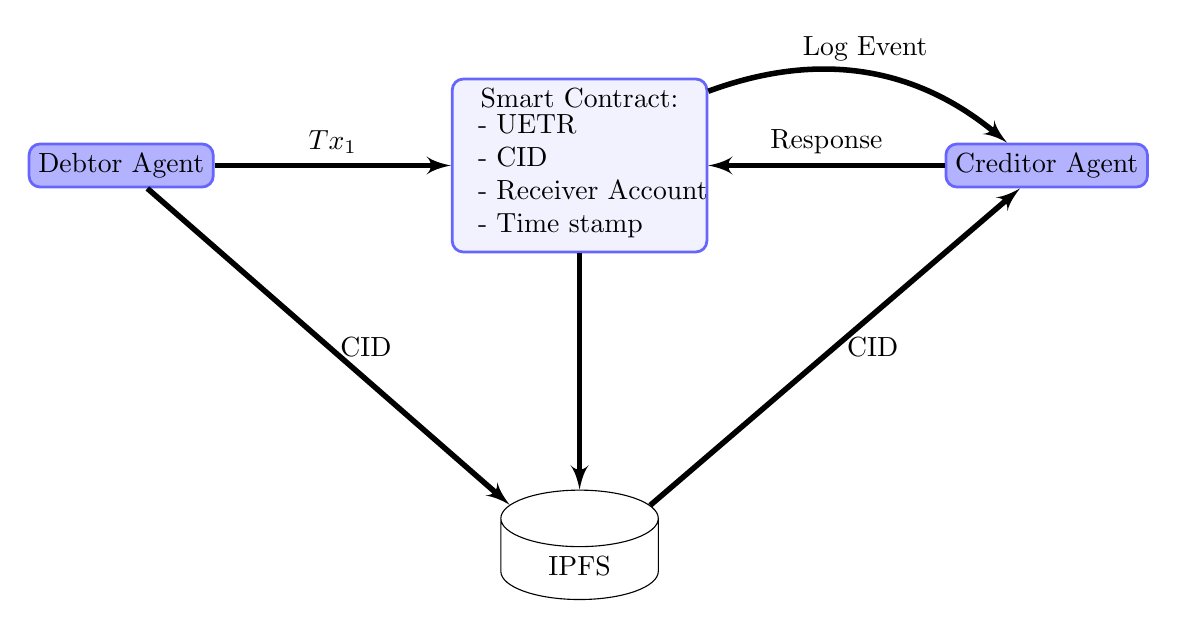
\begin{tikzpicture}[
    block/.style={rectangle, rounded corners, draw=blue!60, fill=blue!5, line width=1pt},
    blockfill/.style={rectangle, rounded corners, draw=blue!60, fill=blue!30, line width=1pt},
    line/.style={draw, -latex', line width=2pt},
    node distance=3cm
]

% Define nodes
\node[blockfill] (debtoragent) {Debtor Agent};
\node[block, right=of debtoragent, text width=3cm, align=center] (smartcontract) {Smart Contract:\\
\begin{tabular}{l}
- UETR\\
- CID\\
- Receiver Account\\
- Time stamp
\end{tabular}};
\node[draw, cylinder, shape aspect=0.7, shape border rotate=90, minimum height=3.0em, minimum width=2.0cm, below=of smartcontract] (ipfs) {IPFS};
\node[blockfill, right=of smartcontract] (creditoragent) {Creditor Agent};

% Connect nodes
\draw [line] (debtoragent) -- node[above] {$Tx_1$} (smartcontract);
\draw [line] (creditoragent) -- node[midway, above, sloped] {Response} (smartcontract);
\draw [line] (debtoragent) -- node[right] {CID} (ipfs);
\draw [line] (ipfs) -- node[right] {CID} (creditoragent);
\draw [line] (smartcontract) -- (ipfs);
\draw [line, bend left=30] (smartcontract) to node[midway, above] {Log Event} (creditoragent);

\end{tikzpicture}
\end{document}
